\documentclass[11pt,a4paper]{article}
\usepackage[utf8]{inputenc}
\usepackage[T1]{fontenc}
\usepackage[french]{babel}
\usepackage{amsmath,amssymb}
\usepackage{booktabs}
\usepackage{graphicx}
\usepackage{hyperref}
\usepackage[margin=2.5cm]{geometry}
\usepackage{caption}
\usepackage{subcaption}

\title{Détection d'hallucinations par Weighted Entropy Production Rate (WEPR)}
\author{Projet StatApp}
\date{}

\begin{document}
\maketitle

% ─────────────────────────────────────────────────────────────
\section{Introduction}

Ce document résume le travail réalisé autour de la méthode WEPR (\emph{Weighted Entropy Production Rate}), proposée par Moslonka \emph{et al.}~\cite{moslonka2026}, pour la détection d'hallucinations dans les grands modèles de langage (LLM). L'idée centrale est d'exploiter les distributions de probabilité sur les top-$K$ tokens à chaque position pour construire un score de confiance au niveau de la séquence.

% ─────────────────────────────────────────────────────────────
\section{Pipeline expérimental}

Le pipeline se décompose en quatre étapes séquentielles.

\paragraph{1. Génération des données.}
On interroge le modèle \texttt{Gemini 2.0 Flash} sur des questions du benchmark TriviaQA, avec les paramètres suivants~: température~$= 1{,}0$, longueur maximale~$= 128$ tokens, $K = 10$ (nombre de tokens candidats renvoyés par position). Pour chaque réponse générée, on stocke les log-probabilités des $K$ candidats à chaque position $j$. Le jeu de données brut contient environ $74\,000$ réponses.

\paragraph{2. Annotation (LLM-as-a-judge).}
Chaque réponse est étiquetée comme \emph{correcte} ou \emph{hallucinée} par un juge LLM (Gemini), avec des règles strictes de correspondance factuelle aux réponses de référence de TriviaQA. Résultat~: $62\,530$ réponses correctes ($84{,}7\,\%$) et $11\,263$ hallucinées ($15{,}3\,\%$).

\paragraph{3. Entraînement du modèle WEPR.}
Une régression logistique est entraînée sur les features WEPR extraites des distributions top-$K$ (détaillées en sections~\ref{sec:methode} et~\ref{sec:training}).

\paragraph{4. Évaluation.}
Les performances sont estimées par bootstrap ($B = 1000$ itérations) et comparées à plusieurs baselines (détails en section~\ref{sec:bootstrap}). Les courbes ROC, PR et les distributions de scores sont générées.

% ─────────────────────────────────────────────────────────────
\section{Méthode}\label{sec:methode}

\subsection{Contributions entropiques}

Pour chaque position $j \in \{1, \dots, L\}$ et chaque rang $k \in \{1, \dots, K\}$, on calcule la contribution entropique~:
\begin{equation}
    s(k, j) = -p(k, j) \log_2 p(k, j),
\end{equation}
où $p(k,j)$ est la probabilité du $k$-ème token le plus probable à la position $j$.

\subsection{EPR (baseline non supervisée)}

L'\emph{Entropy Production Rate} est la moyenne de l'entropie tronquée sur la séquence~:
\begin{equation}
    \text{EPR} = \frac{1}{L} \sum_{j=1}^{L} H_K(j), \qquad H_K(j) = \sum_{k=1}^{K} s(k,j).
\end{equation}
Un EPR élevé indique une incertitude élevée du modèle, donc un risque d'hallucination plus fort.

\subsection{WEPR (score supervisé)}

WEPR pondère les contributions entropiques par des coefficients appris. Le score de séquence est~:
\begin{equation}
    \text{WEPR} = \frac{1}{L} \sum_{j=1}^{L} S_\beta(j) + \sum_{k=1}^{K} \gamma_k \max_j\, s(k,j),
\end{equation}
avec $S_\beta(j) = \beta_0 + \sum_{k=1}^{K} \beta_k\, s(k,j)$.

Le vecteur de features pour la régression logistique est de dimension $2K = 20$~:
\begin{itemize}
    \item $\overline{s}(k) = \frac{1}{L}\sum_j s(k,j)$ pour $k = 1, \dots, K$ (moyennes par rang),
    \item $\max_j s(k,j)$ pour $k = 1, \dots, K$ (maxima par rang).
\end{itemize}

La confiance au niveau de la séquence est $\sigma(\text{WEPR}) \in [0, 1]$, et au niveau du token~: $\sigma(S_\beta(j))$.

% ─────────────────────────────────────────────────────────────
\section{Entraînement}\label{sec:training}

\subsection{Variable cible et formulation}

Le problème est formulé comme une classification binaire. La variable cible est~:
\[
    y_i = \begin{cases} 1 & \text{si la réponse } i \text{ est correcte (non hallucinée),} \\ 0 & \text{si la réponse } i \text{ est hallucinée.} \end{cases}
\]
L'étiquetage est issu du juge LLM (étape 2 du pipeline). Sur les $n = 73\,793$ échantillons retenus (après filtrage des réponses sans verdict), on a $62\,530$ positifs ($y = 1$) et $11\,263$ négatifs ($y = 0$), soit un ratio de déséquilibre d'environ $5{,}6 : 1$.

\subsection{Modèle et loss}

On entraîne une régression logistique \textbf{sans régularisation} (paramètre \texttt{penalty=None} de scikit-learn, équivalent à $C = +\infty$). La fonction de perte minimisée est la \emph{log-loss} (entropie croisée binaire)~:
\begin{equation}
    \mathcal{L}(\theta) = -\frac{1}{n}\sum_{i=1}^{n} \Big[ y_i \log \hat{p}_i + (1 - y_i) \log(1 - \hat{p}_i) \Big],
\end{equation}
où $\hat{p}_i = \sigma(\theta^\top \tilde{x}_i)$ est la probabilité prédite pour l'échantillon $i$, $\tilde{x}_i$ est le vecteur de features standardisé, et $\theta = (\beta_0, \beta_1, \dots, \beta_K, \gamma_1, \dots, \gamma_K)$ regroupe les $2K + 1 = 21$ paramètres du modèle.

\paragraph{Absence de régularisation.}
La régularisation (L1 ou L2) ajoute un terme de pénalité $\lambda \|\theta\|$ à la loss pour empêcher les coefficients de prendre des valeurs trop grandes, ce qui réduit le surapprentissage lorsque le nombre de features est élevé par rapport au nombre d'observations. Ici, on s'en passe pour deux raisons~: (i)~le nombre de paramètres est faible ($2K + 1 = 21$) par rapport au nombre d'échantillons ($n \approx 74\,000$), donc le risque de surapprentissage est limité~; (ii)~l'article original de Moslonka \emph{et al.} n'utilise pas de régularisation, et on reproduit leur protocole. L'absence de régularisation permet aussi une interprétation directe des coefficients $\beta_k$ et $\gamma_k$ sans biais de shrinkage.

\paragraph{Optimisation par L-BFGS.}
L-BFGS (\emph{Limited-memory Broyden--Fletcher--Goldfarb--Shanno}) est un algorithme d'optimisation quasi-newtonien. Contrairement à la descente de gradient classique, qui n'utilise que le gradient (dérivée première) pour mettre à jour les paramètres, L-BFGS approxime la matrice hessienne (dérivées secondes) à partir des derniers gradients calculés, ce qui lui permet de converger plus rapidement. Le préfixe « L » (\emph{limited-memory}) signifie qu'il n'a pas besoin de stocker la hessienne complète en mémoire, ce qui le rend efficace même avec de nombreux paramètres. Ici, avec seulement 21 paramètres et une loss convexe, la convergence est atteinte en quelques itérations (au plus 1000 autorisées).


\subsection{Validation croisée stratifiée}

Les performances sont évaluées par validation croisée stratifiée à $5$ folds (\texttt{StratifiedKFold}, \texttt{seed=42}). Le jeu de données est découpé en 5 parts (folds) de taille à peu près égale. La stratification garantit que chaque fold conserve la même proportion de classes que le jeu complet ($\approx 85\,\%$ positifs / $15\,\%$ négatifs). On réalise ensuite 5 itérations~: à chaque itération, un fold différent sert de jeu de test, et les 4 autres de jeu d'entraînement.

Pour chaque itération~:
\begin{enumerate}
    \item \textbf{Ajustement du scaler.} On calcule la moyenne $\mu_d$ et l'écart-type $\sigma_d$ de chaque feature \emph{uniquement sur les 4 folds d'entraînement}, puis on transforme à la fois les données d'entraînement et de test avec ces valeurs.
    \item \textbf{Entraînement.} La régression logistique est entraînée sur les données d'entraînement standardisées.
    \item \textbf{Évaluation.} L'AUC-ROC est calculée sur le fold de test à partir des probabilités prédites $\hat{p}_i$.
\end{enumerate}
Les AUC par fold sont~: $0{,}683$, $0{,}677$, $0{,}692$, $0{,}678$, $0{,}673$, donnant une moyenne de $\overline{\text{AUC}}_{\text{CV}} = 0{,}681 \pm 0{,}007$.

% ─────────────────────────────────────────────────────────────
\section{Évaluation par bootstrap}\label{sec:bootstrap}

Pour obtenir des intervalles de confiance sur les métriques de performance, on utilise un protocole de \emph{bootstrap} à $B = 1000$ itérations, avec une distinction importante entre les méthodes non paramétriques et la méthode apprise.

\subsection{Baselines non paramétriques (EPR, log-prob, perplexité)}

Pour ces méthodes, le score de chaque séquence est calculé une seule fois de manière déterministe (pas d'entraînement). À chaque itération $b$~:
\begin{enumerate}
    \item On tire un échantillon bootstrap $\mathcal{B}_b$ de taille $n$ \textbf{avec remise} à partir du jeu complet.
    \item On calcule l'AUC-ROC sur cet échantillon~: $\text{AUC}_b = \text{ROC-AUC}(y_{\mathcal{B}_b}, s_{\mathcal{B}_b})$.
\end{enumerate}
On en déduit la moyenne, l'écart-type, et l'intervalle de confiance à $95\,\%$ par les percentiles $2{,}5\,\%$ et $97{,}5\,\%$ de la distribution empirique $\{\text{AUC}_1, \dots, \text{AUC}_B\}$.

\subsection{WEPR (méthode apprise)}

Pour WEPR, le modèle doit être ré-entraîné à chaque itération pour éviter un biais optimiste (le score dépend de données vues à l'entraînement). On utilise un schéma \emph{bootstrap out-of-bag} (OOB)~:
\begin{enumerate}
    \item On tire un échantillon bootstrap $\mathcal{B}_b$ de taille $n$ avec remise.
    \item Les observations \textbf{non tirées} forment l'ensemble OOB $\mathcal{O}_b = \{1, \dots, n\} \setminus \mathcal{B}_b$ (environ $36{,}8\,\%$ des données en espérance).
    \item On ajuste le scaler et la régression logistique ($C = 10^{10} \approx +\infty$) sur $\mathcal{B}_b$.
    \item On calcule $\text{AUC}_b$ sur $\mathcal{O}_b$.
\end{enumerate}
Pour des raisons de temps de calcul, le jeu est sous-échantillonné à $10\,000$ observations avant le bootstrap (tirage sans remise).

Ce protocole explique la plus grande variance de WEPR ($\sigma = 0{,}011$) par rapport aux baselines ($\sigma \approx 0{,}003$)~: chaque itération entraîne un modèle différent sur un échantillon différent, et l'évalue sur un ensemble OOB de taille variable.

% ─────────────────────────────────────────────────────────────
\section{Résultats}

\subsection{Performances comparées}

Le tableau~\ref{tab:results} présente les AUC-ROC obtenues par bootstrap ($B = 1000$).

\begin{table}[h]
\centering
\caption{AUC-ROC par méthode (bootstrap, $B = 1000$, $n = 73\,793$).}
\label{tab:results}
\begin{tabular}{lccc}
\toprule
Méthode & AUC moyenne & Écart-type & IC à 95\,\% \\
\midrule
\textbf{WEPR}       & \textbf{0.682} & 0.0105 & [0.662, 0.702] \\
EPR                  & 0.656          & 0.0029 & [0.650, 0.662] \\
Mean log-prob        & 0.633          & 0.0030 & [0.627, 0.639] \\
Perplexité           & 0.633          & 0.0030 & [0.627, 0.639] \\
Min log-prob         & 0.622          & 0.0029 & [0.616, 0.628] \\
\bottomrule
\end{tabular}
\end{table}

WEPR obtient la meilleure AUC-ROC ($0{,}682$), soit un gain de $+2{,}6$ points par rapport à l'EPR ($0{,}656$) et $+6{,}0$ points par rapport à la perplexité ($0{,}633$). La validation croisée 5 folds donne une AUC cohérente de $0{,}681 \pm 0{,}007$.

On note que WEPR présente un écart-type plus large ($0{,}011$ vs $0{,}003$), ce qui s'explique par le fait que le modèle est ré-entraîné sur chaque échantillon bootstrap (contrairement aux baselines non paramétriques).

\subsection{Courbes ROC et Précision-Rappel}

\begin{figure}[h]
\centering
\begin{subfigure}{0.48\textwidth}
    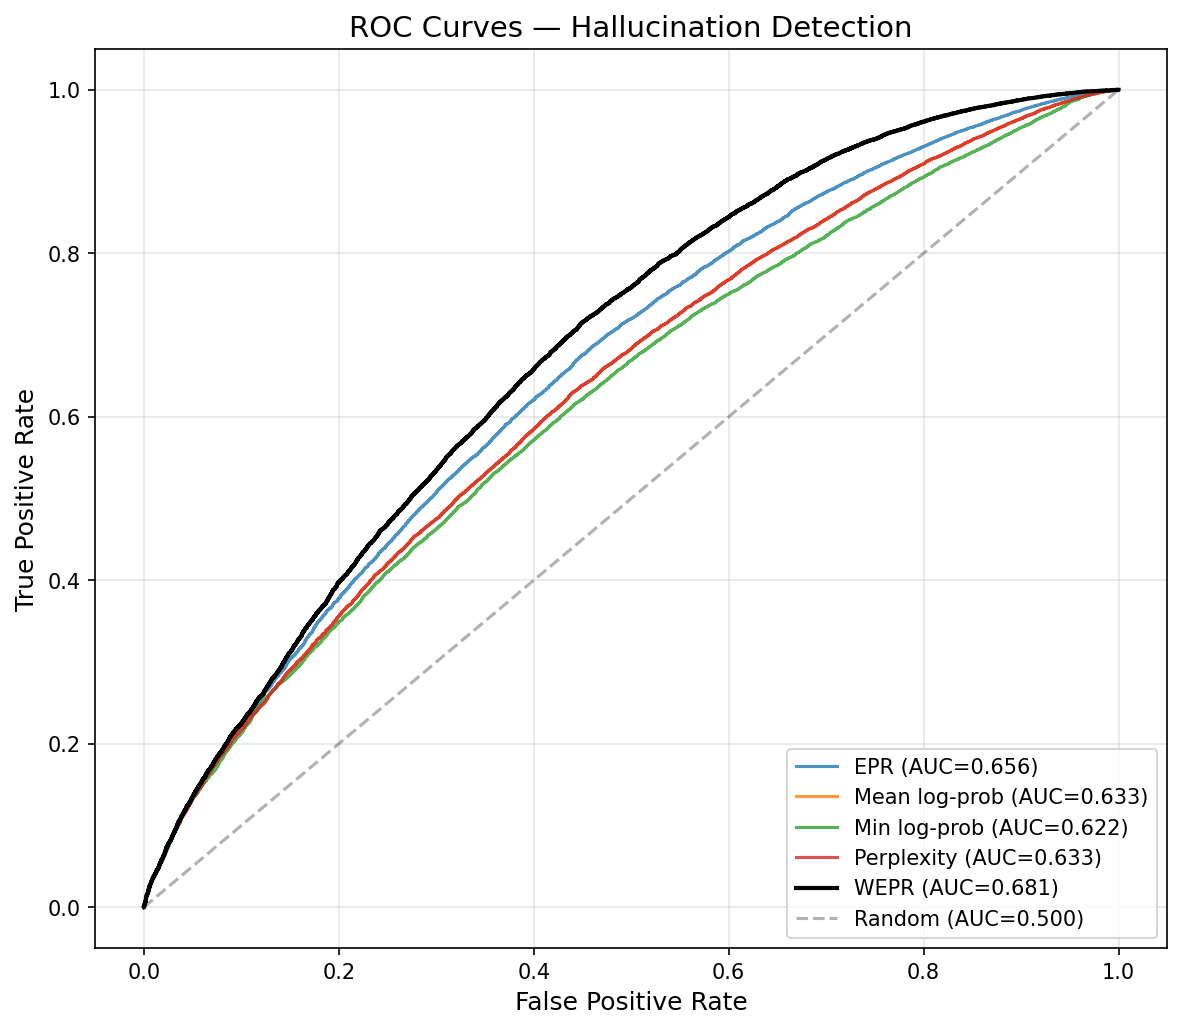
\includegraphics[width=\textwidth]{figures/roc_curves.png}
    \caption{Courbes ROC.}
\end{subfigure}
\hfill
\begin{subfigure}{0.48\textwidth}
    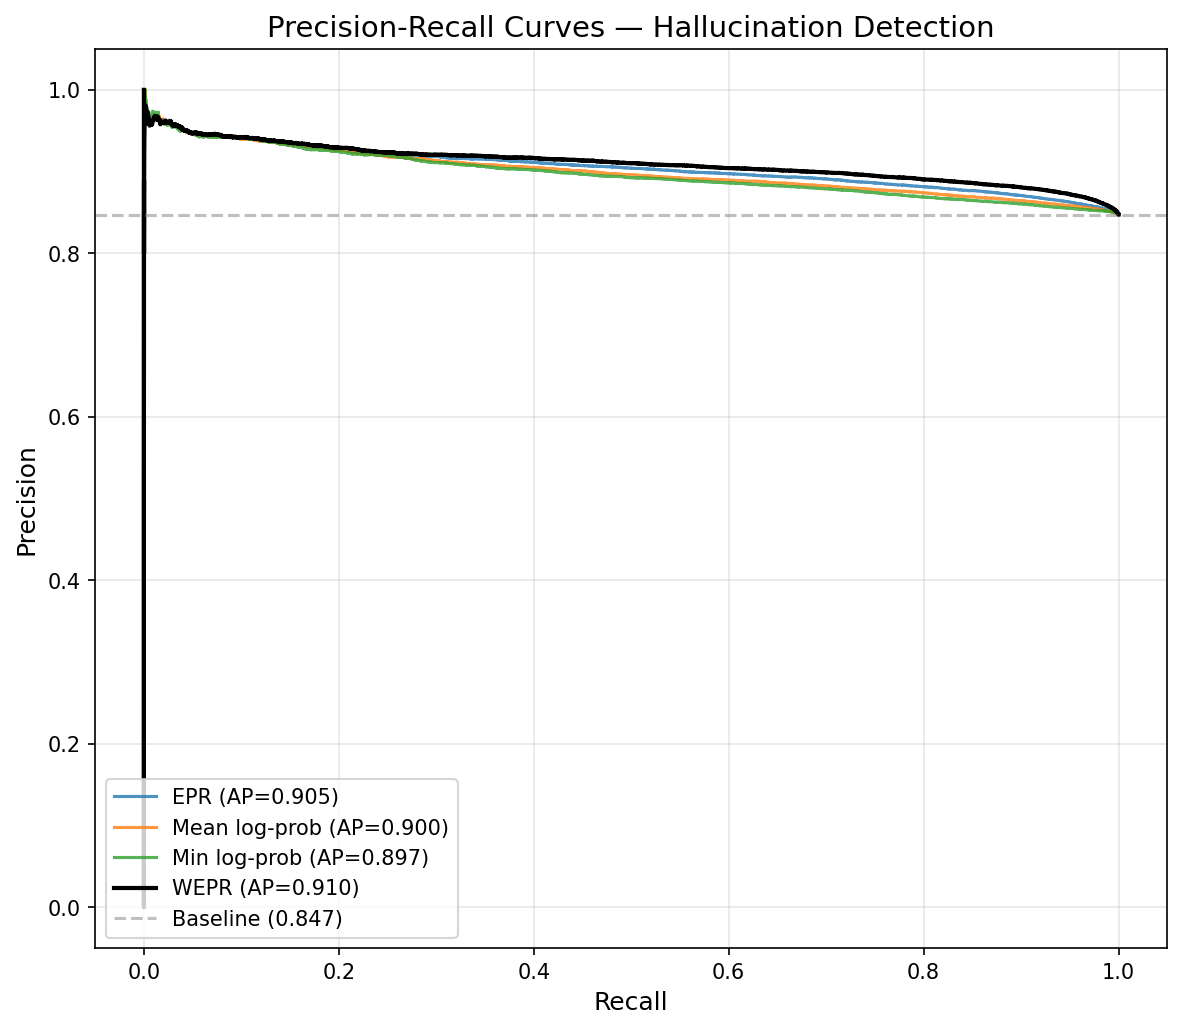
\includegraphics[width=\textwidth]{figures/pr_curves.png}
    \caption{Courbes Précision-Rappel.}
\end{subfigure}
\caption{Comparaison des méthodes de détection d'hallucinations.}
\label{fig:roc_pr}
\end{figure}

La figure~\ref{fig:roc_pr} montre que WEPR domine les autres méthodes sur l'ensemble du spectre ROC. Sur les courbes PR, les écarts sont plus faibles du fait du déséquilibre des classes ($84{,}7\,\%$ de réponses correctes), avec des AP (\emph{Average Precision}) proches entre toutes les méthodes ($\approx 0{,}90$).

\subsection{Distributions de scores et comparaison bootstrap}

\begin{figure}[h]
\centering
\begin{subfigure}{0.48\textwidth}
    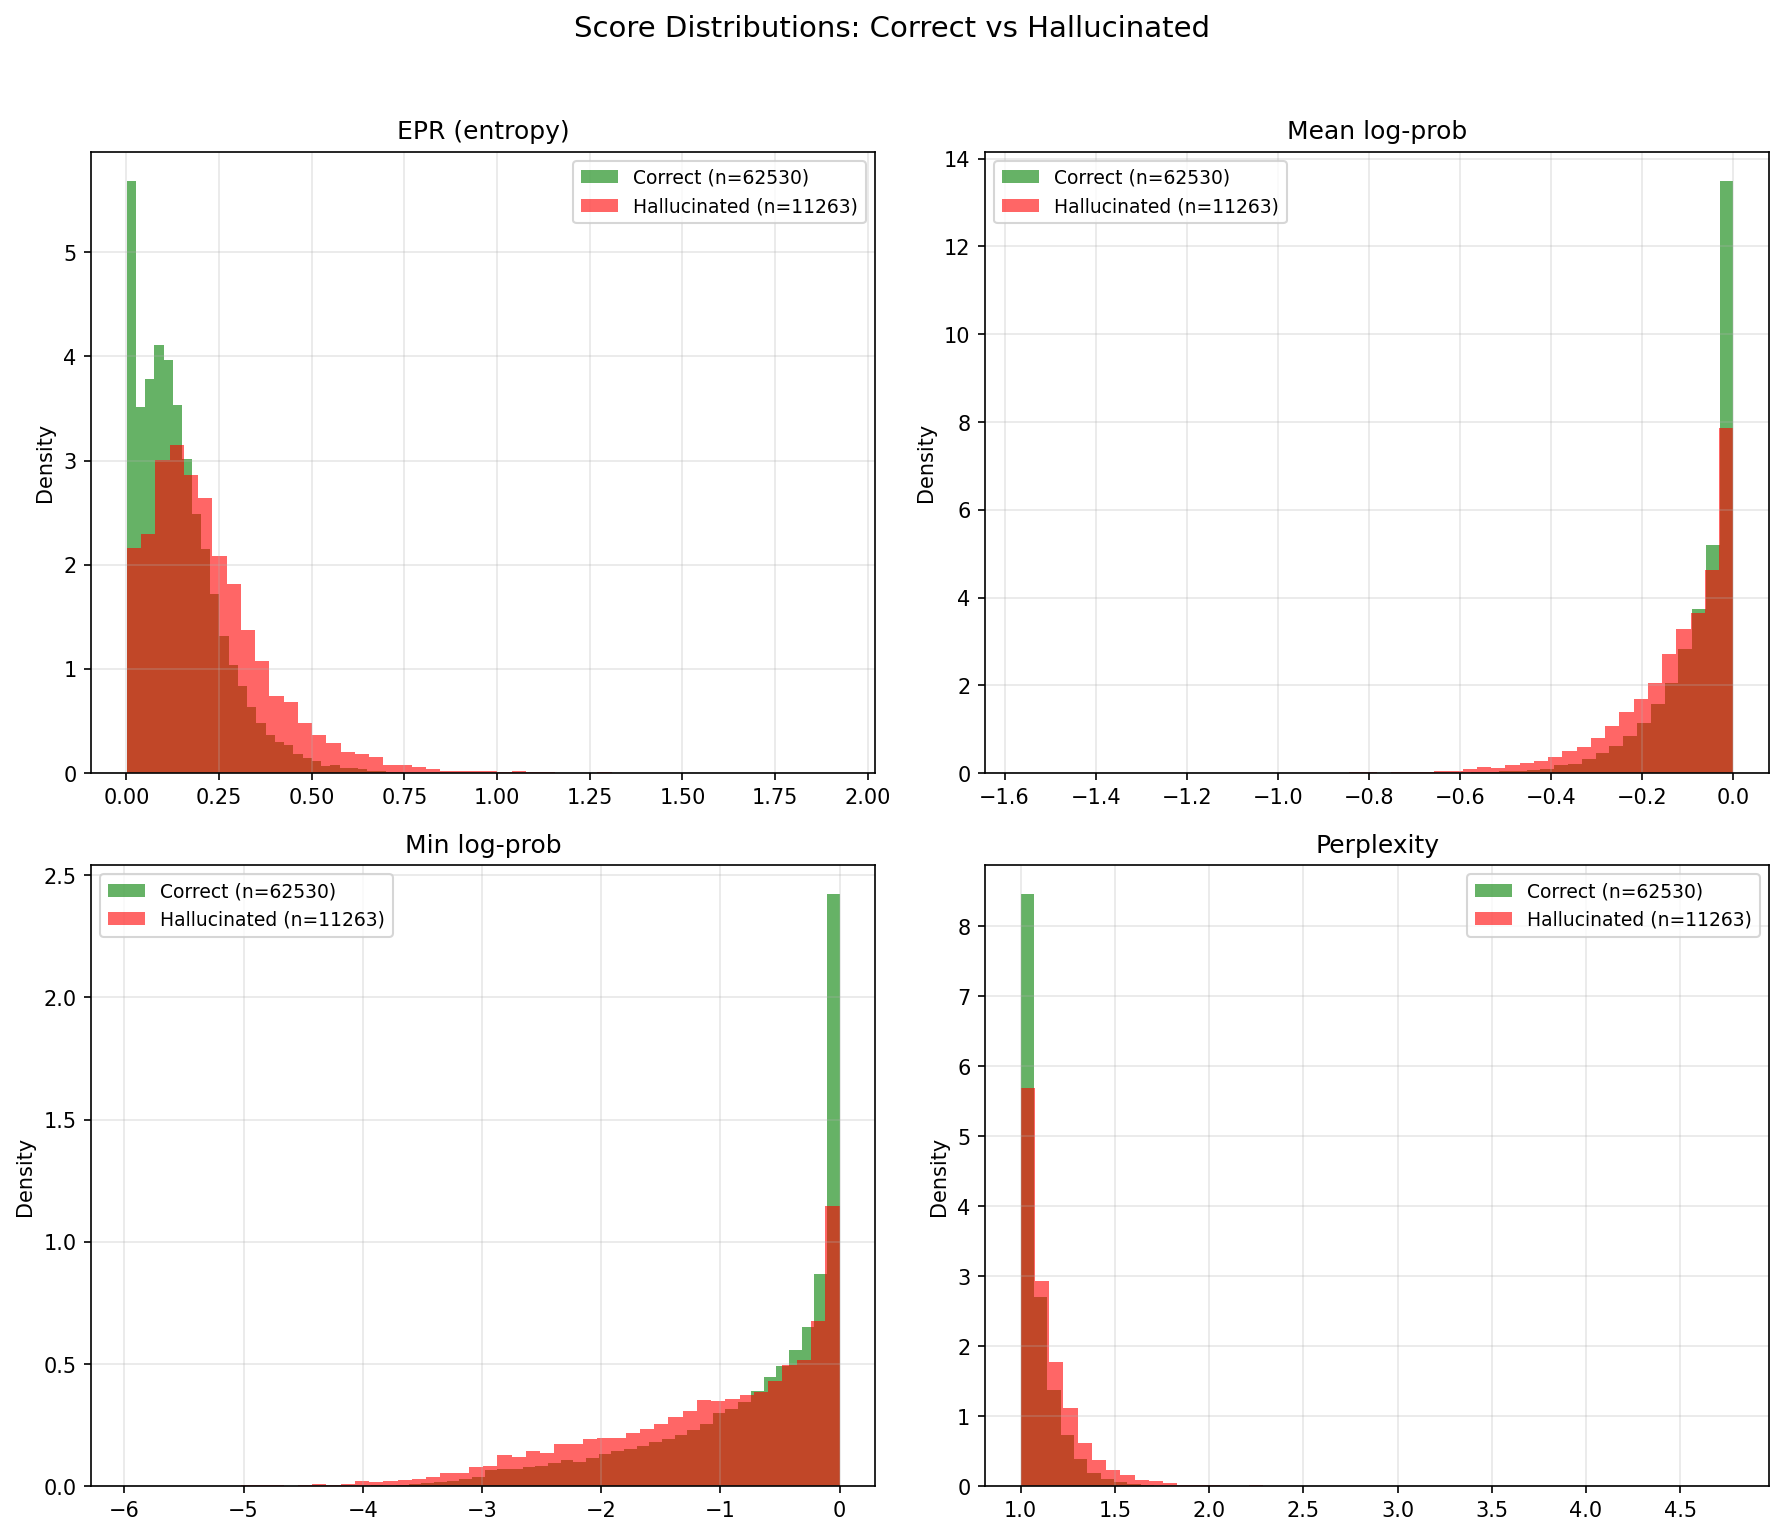
\includegraphics[width=\textwidth]{figures/score_distributions.png}
    \caption{Distributions des scores.}
\end{subfigure}
\hfill
\begin{subfigure}{0.48\textwidth}
    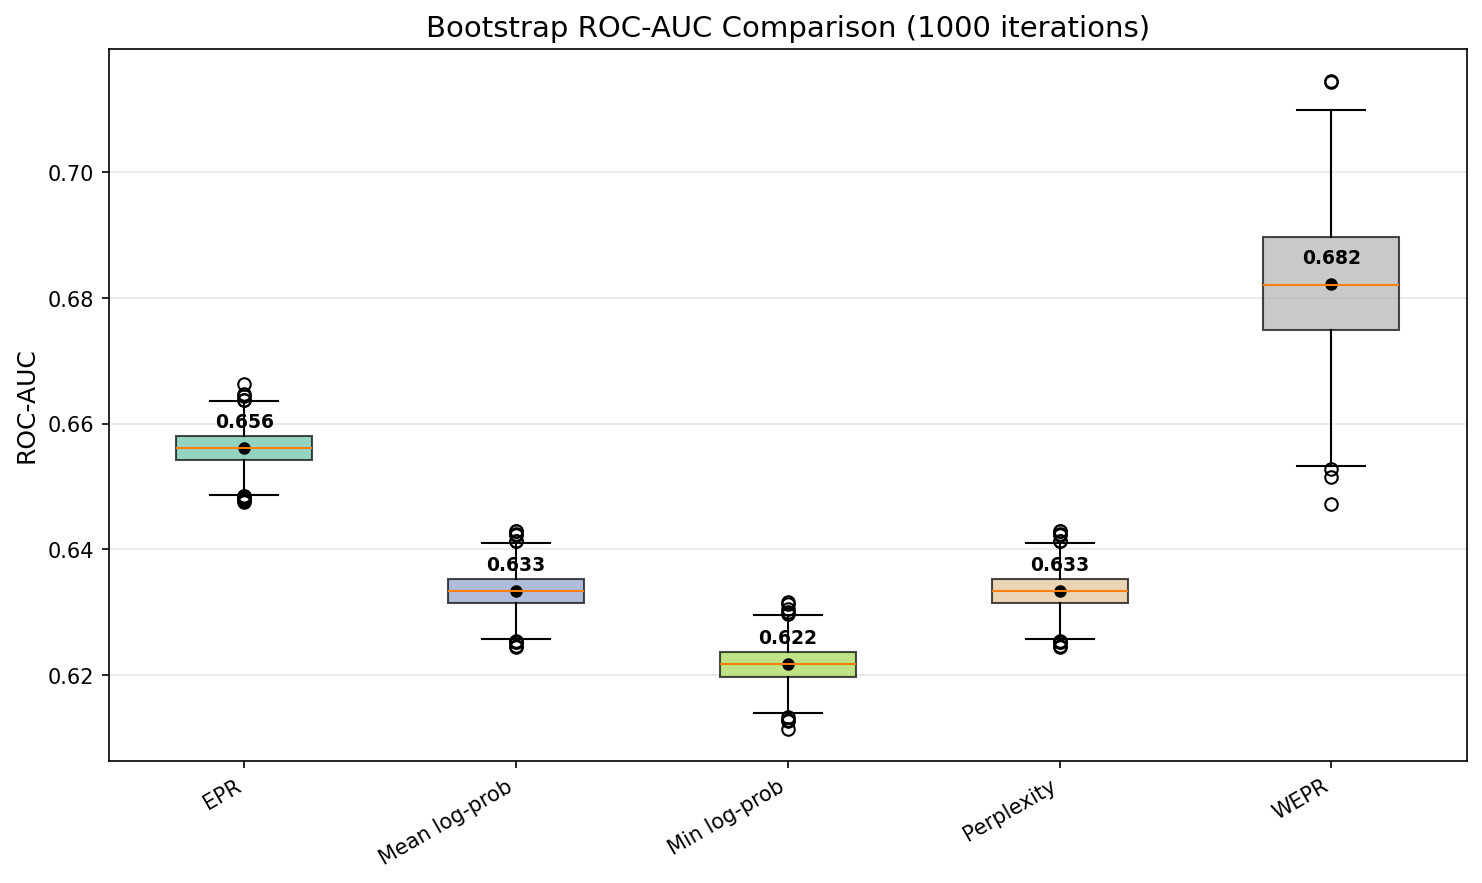
\includegraphics[width=\textwidth]{figures/bootstrap_comparison.png}
    \caption{Comparaison bootstrap des AUC.}
\end{subfigure}
\caption{Analyse des distributions et de la stabilité.}
\label{fig:dist_boot}
\end{figure}

La figure~\ref{fig:dist_boot}(a) montre que les distributions de scores entre réponses correctes et hallucinées se chevauchent fortement pour toutes les méthodes, ce qui explique les AUC modérées. L'EPR offre la meilleure séparation visuelle parmi les baselines.

La figure~\ref{fig:dist_boot}(b) confirme la supériorité de WEPR en termes de moyenne d'AUC, tout en illustrant sa plus grande variance d'estimation.

% ─────────────────────────────────────────────────────────────
\section{Coefficients appris}

Les poids les plus significatifs du modèle entraîné sont~:
\begin{itemize}
    \item $\beta_0 = 1{,}82$ (intercept positif~: biais vers \emph{correct}),
    \item $\beta_1 = 0{,}52$ (rang 1~: plus l'entropie du top-1 est élevée, plus la confiance augmente -- effet contre-intuitif lié à la normalisation),
    \item $\beta_2 = -0{,}56$ (rang 2~: effet négatif fort -- l'entropie sur le deuxième candidat est un signal d'hallucination),
    \item $\gamma_1 = -0{,}19$, $\gamma_{10} = -0{,}17$ (les maxima d'entropie aux rangs extrêmes réduisent la confiance).
\end{itemize}

\paragraph{Interprétation.}
Rappelons que $y = 1$ signifie \emph{correct} et $y = 0$ signifie \emph{halluciné}. Un coefficient positif augmente le score WEPR, donc pousse la prédiction vers \emph{correct}~; un coefficient négatif pousse vers \emph{halluciné}.

L'intercept $\beta_0 = 1{,}82$ est élevé et positif, ce qui reflète le déséquilibre des classes~: avec $84{,}7\,\%$ de réponses correctes, le modèle part avec un a priori fort en faveur de \emph{correct} avant même de regarder les features.

Le signe opposé de $\beta_1$ et $\beta_2$ révèle le signal le plus informatif du modèle. Quand le token de rang~1 (le plus probable) a une entropie élevée ($\beta_1 > 0$), cela signifie que ce token a une probabilité modérée plutôt qu'écrasante -- le modèle distribue sa masse de probabilité, mais le token choisi reste le favori. En revanche, quand le token de rang~2 a aussi une entropie élevée ($\beta_2 < 0$), cela signifie qu'un concurrent sérieux existe avec une probabilité comparable. C'est cette \emph{compétition entre les deux premiers candidats} qui est le marqueur principal d'hallucination~: le LLM hésite entre deux réponses plausibles, signe qu'il n'est sûr d'aucune.

Les coefficients $\gamma_k$ (négatifs pour les rangs extrêmes) indiquent que la présence d'au moins un token dans la séquence où l'entropie aux rangs 1 ou 10 est anormalement élevée est un signal d'alerte, même si le comportement moyen est rassurant. C'est le rôle du terme $\max_j s(k,j)$~: détecter les \emph{pics} d'incertitude locaux.

Les coefficients des rangs intermédiaires ($\beta_3$ à $\beta_{10}$, $\gamma_2$ à $\gamma_9$) sont proches de zéro, ce qui suggère que l'essentiel de l'information discriminante se concentre dans les deux premiers rangs et les comportements extrêmes.

% ─────────────────────────────────────────────────────────────
% ─────────────────────────────────────────────────────────────
\section{Conclusion}

WEPR améliore de manière significative la détection d'hallucinations par rapport aux baselines non supervisées (EPR, perplexité, log-probabilité), avec un gain d'AUC-ROC de $+2{,}6$ points sur l'EPR. La méthode reste cependant limitée en performance absolue (AUC $\approx 0{,}68$), ce qui reflète la difficulté intrinsèque de la tâche en régime boîte noire avec uniquement les top-$K$ log-probabilités.

\begin{thebibliography}{1}
\bibitem{moslonka2026} C. Moslonka \emph{et al.}, ``Learned Hallucination Detection in Black-Box LLMs using Token-level Entropy Production Rate,'' \emph{arXiv:2509.04492v2}, 2026.
\end{thebibliography}

\end{document}
